\chapter{Voltage regulation}\label{ch:voltageRegulation}
%**********************************************

%**********************************************
\section{Introduction} \label{sec:voltIntro}
%**********************************************

Given a 9 $\mathrm{V_{DC}}$ battery, a voltage regulator is required to reduce the voltage level to 5 $\mathrm{V_{DC}}$, as this is the level required by the operational amplifiers used in the rest of the circuit. Two voltage regulators were considered: the LM7805 linear regulator as well as the LM2595 switchmode regulator, which were both analysed with regards to efficiency and noise by means of calculations and simulations. According to the literature, the linear regulator produces insignificant levels of noise, but has low power efficiency of around $50\%$ for input and output of 9 $\mathrm{V_{DC}}$ and 5 $\mathrm{V_{DC}}$\cite{lm7805} respectively. The switchmode regulator can provide power efficiency of around $85\%$, but outputs a considerable amount of noise\cite{lm2595}. With the aforementioned in mind, both of the regulators were simulated (Section \ref{sec:voltDesign}) to determine the best trade-off between low noise and efficiency.

%**********************************************
\section{Design} \label{sec:voltDesign}
%**********************************************

\begin{wrapfigure}{r}{0.5\textwidth}
	\vspace{-1.3cm}
    \centering
    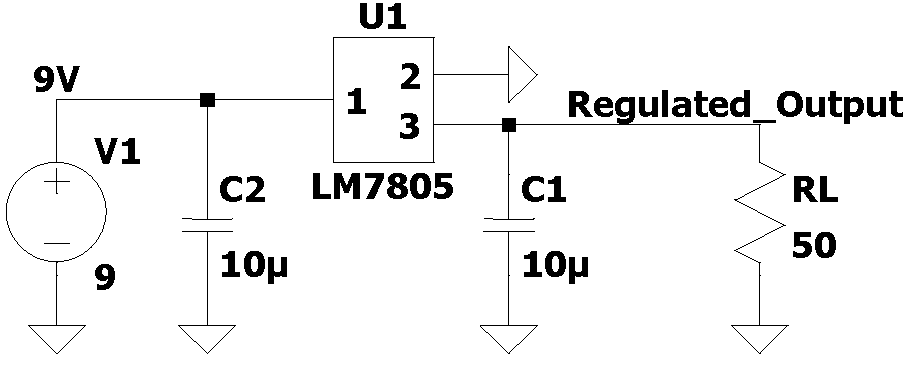
\includegraphics[width = 0.48\textwidth]{Figures/LR.pdf}
    \caption{Linear Voltage Regulator}
    \label{fig:LR}
\end{wrapfigure}

The LM7805 chip and its required peripheral circuit is shown in Figure \ref{fig:LR}. Component values were obtained from the datasheet \cite{lm7805}. For testing purposes, a \SI{50}{\Omega} load was connected to the regulator, drawing \SI{100}{mA}.\\

The LM2595 chip is shown in figure \ref{fig:SM}, built into the required peripheral circuit. Capacitor and inductor values were obtained from the datasheet \cite{lm2595}. Resistor values were calculated:

$$\mathrm{V}_{\mathrm{OUT}}=\mathrm{V}_{\mathrm{REF}}\left(1+\frac{\mathrm{R}_{2}}{\mathrm{R}_{1}}\right) \quad \text { where } \mathrm{V}_{\mathrm{REF}}=1.23 \mathrm{V}$$

Selecting $\mathrm{R_1}$ as \SI{1}{\kilo\Omega}, with $\mathrm{V_{out}}$ as \SI{5}{\volt} gives $\mathrm{R_2}$ as \SI{3065}{\Omega}. For testing purposes, a \SI{50}{\Omega} load was connected to the regulator, drawing \SI{100}{mA}.\\
\pagebreak 

\begin{wrapfigure}{r}{0.7\textwidth}
%\begin{figure}
%	\vspace{1.2cm}
    \centering
    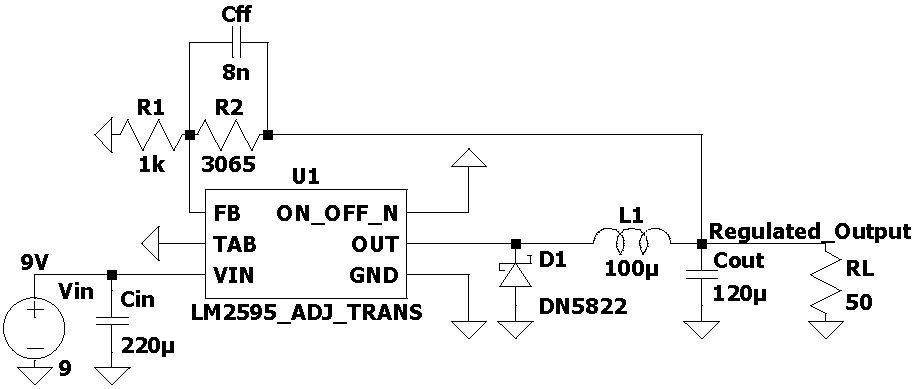
\includegraphics[width = 0.72\textwidth]{Figures/SM.pdf}
    \caption{Switchmode Voltage Regulator}
    \label{fig:SM}
\end{wrapfigure}
%\end{figure}

Since the provided circuit includes a resistor ($R_{sense}$) between the voltage source and the voltage regulator, the voltage drop over the resistor will be $V = IR = (0.01238)(0.01) = 123.8\mu \mathrm{V}$. Considering that the power source supplies \SI{9}{V}, the aforementioned voltage drop is negligible - it is not nearly enough to approach the dropout voltages of the voltage regulators, which are \SI{6.7}{\volt} for the LM7805 and \SI{5.8}{\volt} for the LM2595 in the case of a \SI{5}{\volt} output.

%**********************************************
\section{Results} \label{sec:volt_results}
%**********************************************

The input and output power measurements are displayed in table \ref{tab:compvreg}. Comparing the efficiency of the respective regulators, it is clear that the switchmode regulator is considerably more efficient. However, simulation results in a settling time of \SI{1.24}{ms}, which is quite slow. 

\begin{wraptable}{r}{0.75\textwidth}
        \centering
        \footnotesize
        \caption{Comparison of Voltage Regulators}
         \begin{tabular}{c@{\qquad}rrrrr}
          \toprule
             & $I_{in}$ [mA] & $I_{out}$ [mA] & $P_{in}$ [mW] & $P_{out}$ [mW] & $\eta$ [\%] \\
          \midrule
          LM7805 	& 105.06 	& 100.05 	& 945.54 	& 500.55 	& 52.93\\
          LM2595 	& 57.54 	& 99.65 	& 517.86 	& 496.6 	& 95.89\\
          \bottomrule
        \end{tabular}
     \label{tab:compvreg}
\end{wraptable}

Furthermore, the switchmode regulator creates noise levels of up to 950 $\mu V_{pp}$ in the output, as can be seen in figure \ref{fig:smnoise}, whereas the linear regulator produces almost no noise (figure \ref{fig:lmout}). Noise is a problem, as the large gain of the differential amplifier  will increase the noise levels, which will distort the output. 

\begin{figure}[h]
    \centering
    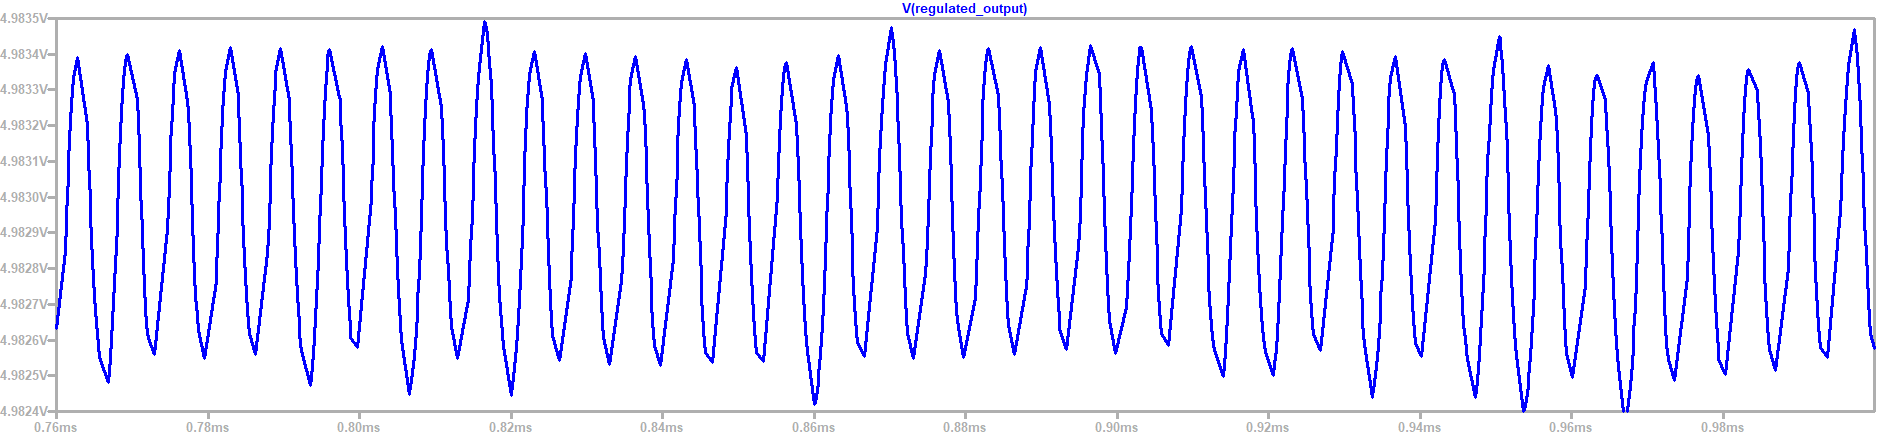
\includegraphics[width = 1\textwidth]{Figures/smnoise.png}
    \caption{Switchmode Voltage Regulator Noise}
    \label{fig:smnoise}
\end{figure}


The output graphs of the voltage regulators are shown in figures \ref{fig:lmout} and \ref{fig:smout}, and clearly demonstrate that both regulators produce the desired output current and voltage. The input current for the switchmode regulator is not shown as it obscures the graph, but it has an average value of \SI{57.54}{mA}. All relevant values can be found in table \ref{tab:compvreg}.

\begin{figure}[h]
    \centering
    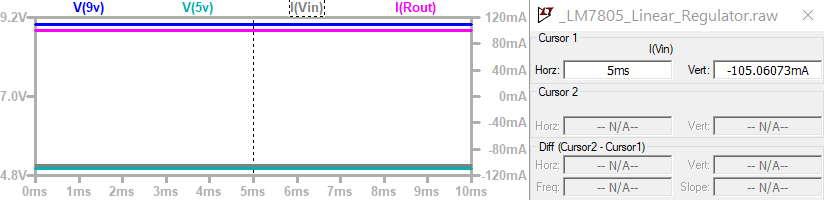
\includegraphics[width = 1\textwidth]{Figures/lmout.png}
    \caption{Linear Voltage Regulator Output}
    \label{fig:lmout}
\end{figure}

\begin{figure}[h]
    \centering
    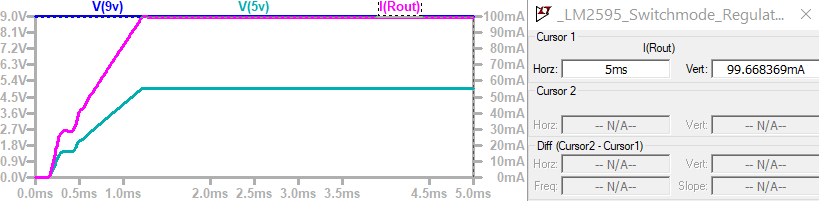
\includegraphics[width = 1\textwidth]{Figures/smout.png}
    \caption{Switchmode Voltage Regulator Output}
    \label{fig:smout}
\end{figure}

%**********************************************
\section{Summary}\label{sec:temp_summary}
%**********************************************
Concluding, it has been shown that both regulators behave as expected, but that the levels of noise present in the switchmode regulator make it unsuitable for the design at hand, as input signals, and thus the noise as well, will be amplified to levels of noise in the output signal that are unacceptable for an ADC input. The linear regulator will therefore be used. This choice was made despite the fact that the switchmode regulator is approximately 40\% more efficient than the linear regulator. However, since the total current drawn is still very low, efficiency is not of concern.